\providecommand{\main}{..}
\documentclass[\main/Apuntes_PL.tex]{subfiles}

  % !TEX root = ../Apuntes_PL.tex

\begin{document}
  \begin{tikzpicture}
    \node[rectangle, draw = black, align = center, rectangle split, rectangle split horizontal, rectangle split parts = 2] (cl1) {};
    \node[rectangle, draw = black, right = .2 of cl1, align = center, rectangle split, rectangle split horizontal, rectangle split parts = 2] (cl2) {};
    \node[rectangle, draw = black, right = .2 of cl2, align = center, rectangle split, rectangle split horizontal, rectangle split parts = 2] (cl3) {};

    \node[unit, right = of cl3, align = center] (ansi) {Analizador\\sintáctico};
    \node[err, below=of ansi] (err) {error};

    \node[rectangle, right=2of ansi, label={Árbol incontextual}] (t1) {$e_0$};
    \node[rectangle, below left =.5 of t1] (t2) {$e_1$};
    \node[rectangle, below right =.5 of t1] (t3) {$e_2$};
    \node[rectangle, below left =.5 of t3] (t4) {$e_3$};
    \node[rectangle, below right =.5 of t3] (t5) {$e_4$};
    \node[rectangle, below left =.5 of t4] (t6) {$e_5$};
    \node[rectangle, below right =.5 of t4] (t7) {$e_6$};
    \node[rectangle, below left =.5 of t7] (t8) {$e_7$};
    \node[rectangle, below right =.5 of t7] (t9) {$e_8$};

    \draw[myarrow] (cl3.east) -- ++(0,0) -> (ansi.west);
    \draw[myarrow] (ansi.south) -- ++(0,0) -> (err.north);
    \draw[myarrow] (ansi.east) -- ++(0,0) -> (t1.west);

    \path[thick]
      (t1.south)  edge (t2)
                  edge (t3)
      (t3.south)  edge (t4)
                  edge (t5)
      (t4.south)  edge (t6)
                  edge (t7)
      (t7.south)  edge (t8)
                  edge (t9);
  \end{tikzpicture}

  \bigskip
  \par
  Hipótesis: Las cadenas de clases léxicas generadas por el analizador léxico forman un lenguaje incontextual.

  \section{Recordatorio}
    \subsection{Gramática}
      Sea una GI (Gramática Incontextual), GI(N,T,P,S):
      \begin{itemize}
        \item N $\equiv$ alfabeto de no terminales $\Rightarrow$ clases sintácticas.
        \item T $\equiv$ alfabeto de terminales $\Rightarrow$ clases léxicas.
        \item P $\equiv$ conjunto de reglas de la forma A $\rightarrow$ $\alpha$, donde A $\in$ N y $\alpha$ $\in$ (NUT)$\ast$.
        \item S $\in$ N y es el símbolo inicial.
      \end{itemize}

      \bigskip
      \par
      Sea G $\equiv$ (N,T,P,S) $\rightarrow$ G denota un lenguaje L(G)
      \begin{itemize}
        \item Relación de derivación $\Rightarrow_G$ (0 $\Rightarrow$ si G se sobreentiende) $\Rightarrow$ $\subseteq$ (NUT)$\ast$ x (NUT)$\ast$\\
              \hspace{5mm}$\alpha$A$\beta$ $\wedge$ A $\rightarrow \gamma \in$ P entonces $\alpha$A$\beta \Rightarrow \alpha \gamma$B
        \item Se considera $\Rightarrow_\ast$ aplicar cero o más veces $\Rightarrow$.
      \end{itemize}

      \par
      L(G) = \{w $\in$ T$\ast$ $\mid$ S $\Rightarrow_\ast$ w\}

      \bigskip
      \par
      \textbf{e.g.} Número binario\\
      \hspace{5mm}N = \{N,B\}\\
      \hspace{5mm}T = \{0,1\}\\
      \hspace{5mm}P = {\color{blue}N} $\rightarrow$ B\\
      \hspace{13mm}{\color{blue}N} $\rightarrow$ NB\\
      \hspace{13mm}{\color{blue}B} $\rightarrow$ {\color{red}0}\\
      \hspace{13mm}{\color{blue}B} $\rightarrow$ {\color{red}1}\\
      \hspace{5mm}S = N\\
      \vspace{2mm}
      \hspace{5mm}Esto sería equivalente a dar tan solo las reglas(P), donde:
      \begin{itemize}
        \item El símbolo {\color{blue}azul} de la primera regla es el símbolo inicial(S).
        \item El conjunto de símbolos {\color{blue}azules} son los no terminales(N).
        \item El conjunto de símbolos {\color{red}rojos} son los terminales(T).
      \end{itemize}

      \bigskip
      \par
      La derivación se denomina \textit{mas a la izquierda} si siempre se reescribe el no terminal que está mas a la izquierda, equivalente para \textit{mas a la derecha}.\\
      \vspace{3mm}
      \hspace{5mm}\textbf{Derivación}\\
      \hspace{10mm}{\color{red}N} $\Rightarrow$ {\color{red}N}B $\Rightarrow$ N{\color{red}B}B $\Rightarrow$ {\color{red}N}1B $\Rightarrow$ B1{\color{red}B} $\Rightarrow$ {\color{red}B}10 $\Rightarrow$ 010\\
      \vspace{3mm}
      \hspace{5mm}\textbf{Derivación mas a la izquierda}\\
      \hspace{10mm}{\color{red}N} $\Rightarrow$ {\color{red}N}B $\Rightarrow$ {\color{red}N}BB $\Rightarrow$ {\color{red}B}BB $\Rightarrow$ 0{\color{red}B}B $\Rightarrow$ 01{\color{red}B} $\Rightarrow$ 010\\
      \vspace{3mm}
      \hspace{5mm}\textbf{Derivación mas a la derecha}\\
      \hspace{10mm}{\color{red}N} $\Rightarrow$ N{\color{red}B} $\Rightarrow$ {\color{red}N}0 $\Rightarrow$ N{\color{red}B}0 $\Rightarrow$ {\color{red}N}10 $\Rightarrow$ {\color{red}B}10 $\Rightarrow$ 010

    \subsection{Árbol de análisis sintáctico}
      \par
      La idea es obtener una representación única para cada sentencia.

      \bigskip
      \par
      \textbf{Árboles}
      \begin{itemize}
        \item La raíz está etiquetada con el símbolo inicial.
        \item Están ordenados, hay un órden en los hijos de los nodos (primer hijo, segundo hijo...).
        \item Los nodos internos están etiquetados por no terminales.
        \item Los nodos hoja están etiquetados por terminales o por $\epsilon$.
        \item Si un nodo está etiquetado por A y sus hijos por $\alpha$ entonces A $\rightarrow \alpha \in$ P.
      \end{itemize}

      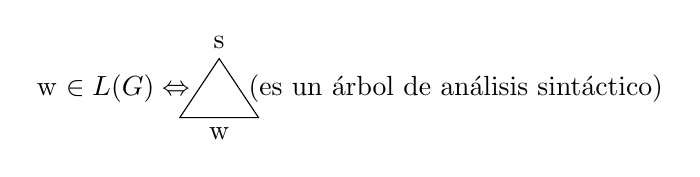
\begin{tikzpicture}
        \draw (0,0) node{}
          -- node[below]{w} (1,0) node{}
          -- node[right]{(es un árbol de análisis sintáctico)} (.5,.75) node[anchor=south]{s}
          -- node[left]{w $\in L(G) \Leftrightarrow$} cycle;
      \end{tikzpicture}

      \par
      \textbf{e.g.}\\
      \begin{center}
        \begin{minipage}{.2\textwidth}
          N $\rightarrow$ B\\
          N $\rightarrow$ NB\\
          B $\rightarrow$ 0\\
          B $\rightarrow$ 1
        \end{minipage}%
        \begin{minipage}{.3\textwidth}
          \begin{tikzpicture}
            \node[rectangle] (t1) {N};
            \node[rectangle, below left =.5 of t1] (t2) {N};
            \node[rectangle, below right =.5 of t1] (t3) {B};
            \node[rectangle, below left =.5 of t2] (t4) {N};
            \node[rectangle, below right =.5 of t2] (t5) {B};
            \node[rectangle, below =.5 of t3] (t6) {0};
            \node[rectangle, below =.5 of t4] (t7) {B};
            \node[rectangle, below =.5 of t5] (t8) {1};
            \node[rectangle, below =.5 of t7] (t9) {0};

            \path[thick]
              (t1.south) edge (t2)
                          edge (t3)
              (t2.south) edge (t4)
                          edge (t5)
              (t3.south) edge (t6)
              (t4.south) edge (t7)
              (t5.south) edge (t8)
              (t7.south) edge (t9);
          \end{tikzpicture}
        \end{minipage}%
        \begin{minipage}{.4\textwidth}
          \raggedright
          Cada nodo es equivalente a un array en el que se referencian sus hijos en orden.
        \end{minipage}
      \end{center}

  \section{Especificación sintáctica}
    \subsection{Determinar las clases sintácticas}
      \par
      ¿Cómo? A partir de la especificación informal.

      \bigskip
      \par
      De arriba a abajo:
      \begin{itemize}
        \item Identificar las clases complejas.
        \item Descomponerlas en clases más simples hasta llegar a las clases léxicas.
      \end{itemize}

      \bigskip
      \par
      Descomposición $\rightarrow$ Las clases resultantes deben estar al mismo nivel, el más alto posible.

      \bigskip
      \par
      \textbf{e.g.} L que describe libros
      \begin{center}
        \begin{minipage}{.4 \textwidth}
          \hspace*{5mm}Titulo [...]\\
          \hspace*{5mm}Autores [Autor]...[Autor]\\
          \hspace*{5mm}Capitulo [...][...]\\
          \hspace*{5mm}...\\
          \hspace*{5mm}Capitulo [...][...]
        \end{minipage}%
        \begin{minipage}{.5 \textwidth}
          \begin{tikzpicture}
            \node[rectangle] (lib) {Libro};
            \node[rectangle, below left =.5 of lib] (cab) {Cabecera};
            \node[rectangle, below right =.5 of lib] (cuer) {Cuerpo};
            \node[rectangle, below left =.5 of cab] (tit) {Titulo};
            \node[rectangle, below right =.5 of cab] (auts) {Autores};
            \node[rectangle, below =.5 of cuer] (cap) {Capitulo};
            \node[rectangle, below =.5 of auts] (aut) {Autor};
            \node[rectangle, below=.5 of cap] (tcap) {TituloCap};
            \node[rectangle, right=.5 of tcap] (ccap) {ContenidoCap};

            \path[thick]
              (lib.south) edge (cab)
                          edge (cuer)
              (cab.south) edge (tit)
                          edge (auts)
              (cuer.south) edge (cap)
              (auts.south) edge (aut)
              (cap.south) edge (tcap)
                          edge (ccap);
          \end{tikzpicture}
        \end{minipage}
      \end{center}
\end{document}